\begin{frame}{Introduction}
\small
\begin{itemize}
    \item Tree-based methods involve \textit{stratifying} or \textit{segmenting} the predictor space into a number of simple regions. \pause

    \item To make a prediction, we use the mean or the mode for the training observations in the region to which it belongs. \pause 

    \item Let's begin with an example... 

    \item Let's predict a baseball player's \textbf{Salary} based on the \textbf{years} that he has played in the major leagues and the \textbf{hits} that he made in the previous year. 

    \end{itemize}
\end{frame}

\begin{frame}{Introduction}

    \begin{figure}
        \centering
        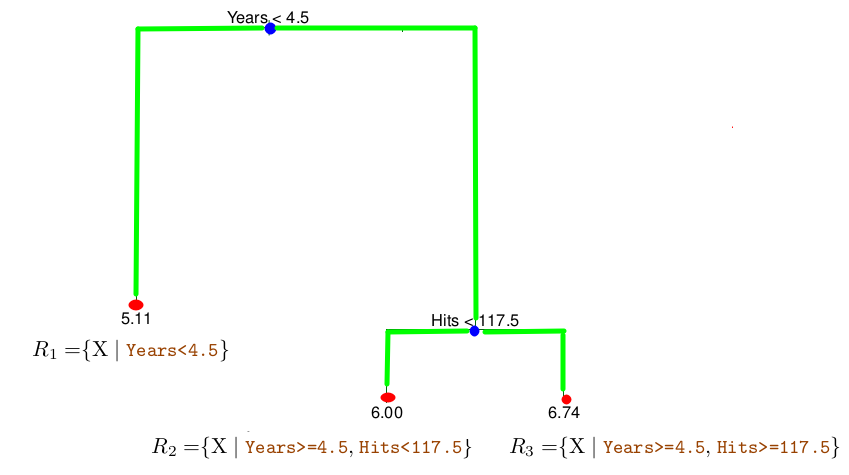
\includegraphics[height=5cm]{introduction/trees.png}
    \end{figure}
\begin{itemize}

\item[\textcolor{red}{$\bullet$}] Terminal nodes or leaves. 
\item[\textcolor{blue}{$\bullet$}]Internal nodes. 
\item[\textcolor{green}{$\bullet$}] Branches. 
\end{itemize}

\end{frame}






